
\subsection{Idealisiertes zonales und meridionales Windfeld}

In der Meteorologie werden Windgeschwindigkeiten in ein rechtwinkliges Koordinatensystem zerlegt. 
Die {zonal}e Komponente \(u\) beschreibt die Geschwindigkeit in Ost-West-Richtung, 
die {meridional}e Komponente \(v\) jene in Nord-Süd-Richtung. 
Positive Werte von \(u\) stehen für eine Strömung nach Osten, positive Werte von \(v\) für eine Strömung nach Norden.


Abbildung~\ref{fig:zonal_wind} zeigt ein idealisiertes zonales Windfeld, bei
dem ausschliesslich eine Ost-West-Strömung vorliegt (\(v = 0\)). Die
Geschwindigkeit hängt von der geographischen Breite \(\theta\) ab und folgt der
Beziehung
\begin{equation}
	u = U_0 \cdot \sin^2(\theta).
	\label{rossby:eq:zonal_wind}
\end{equation}
Ein Druckgradient oder eine vertikale Struktur sind nicht berücksichtigt, es handelt sich um ein rein theoretisches, horizontal homogenes Modell.

\begin{figure}
	\centering
	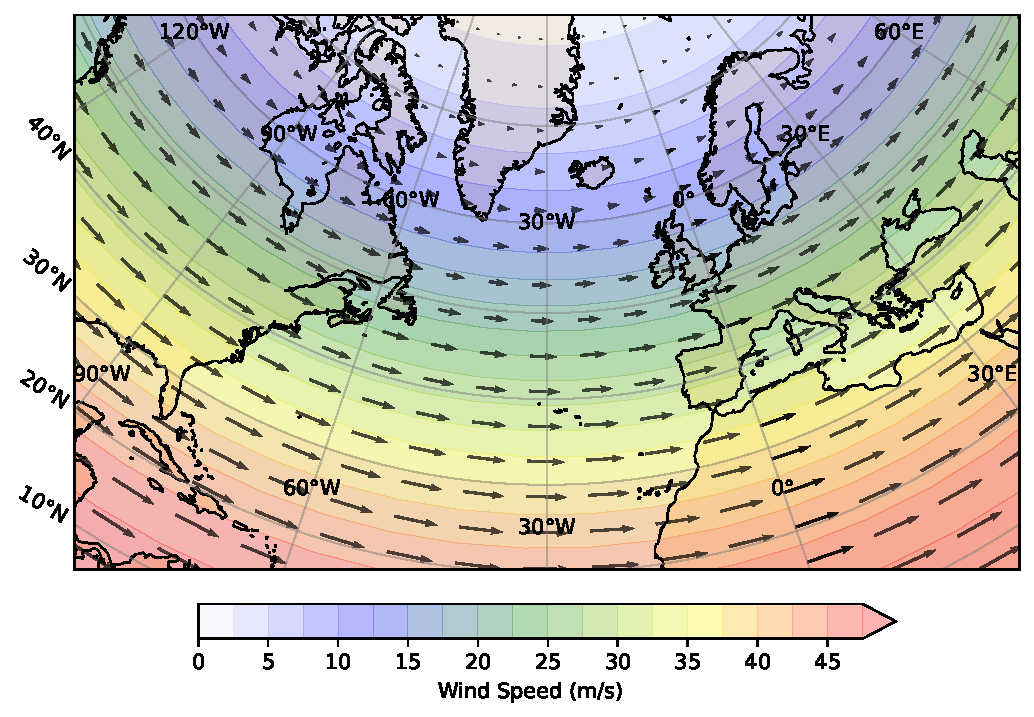
\includegraphics[width=\textwidth, trim=1cm 0cm 2cm 0cm, clip]{papers/rossby/images/zonal_wind_plot.pdf}
	\caption{Idealisiertes zonales Windfeld (\(v=0\)), Geschwindigkeit \(u = U_0 \cdot \sin^2(\theta)\).}
	\label{fig:zonal_wind}
\end{figure}

\noindent
Abbildung~\ref{fig:meridional_wind} zeigt dagegen ein idealisiertes meridionales Windfeld, bei dem nur eine Nord-Süd-Strömung existiert (\(u = 0\)).
Die Geschwindigkeit hängt hier von der Breite ab nach
\begin{equation}
	v = V_0 \cdot \cos(\theta).
	\label{rossby:eq:meridional_wind}
\end{equation}
Auch dieses Feld ist frei von Druckgradienten und vertikaler Struktur und dient der isolierten Betrachtung meridionaler Strömungskomponenten.

\begin{figure}
	\centering
	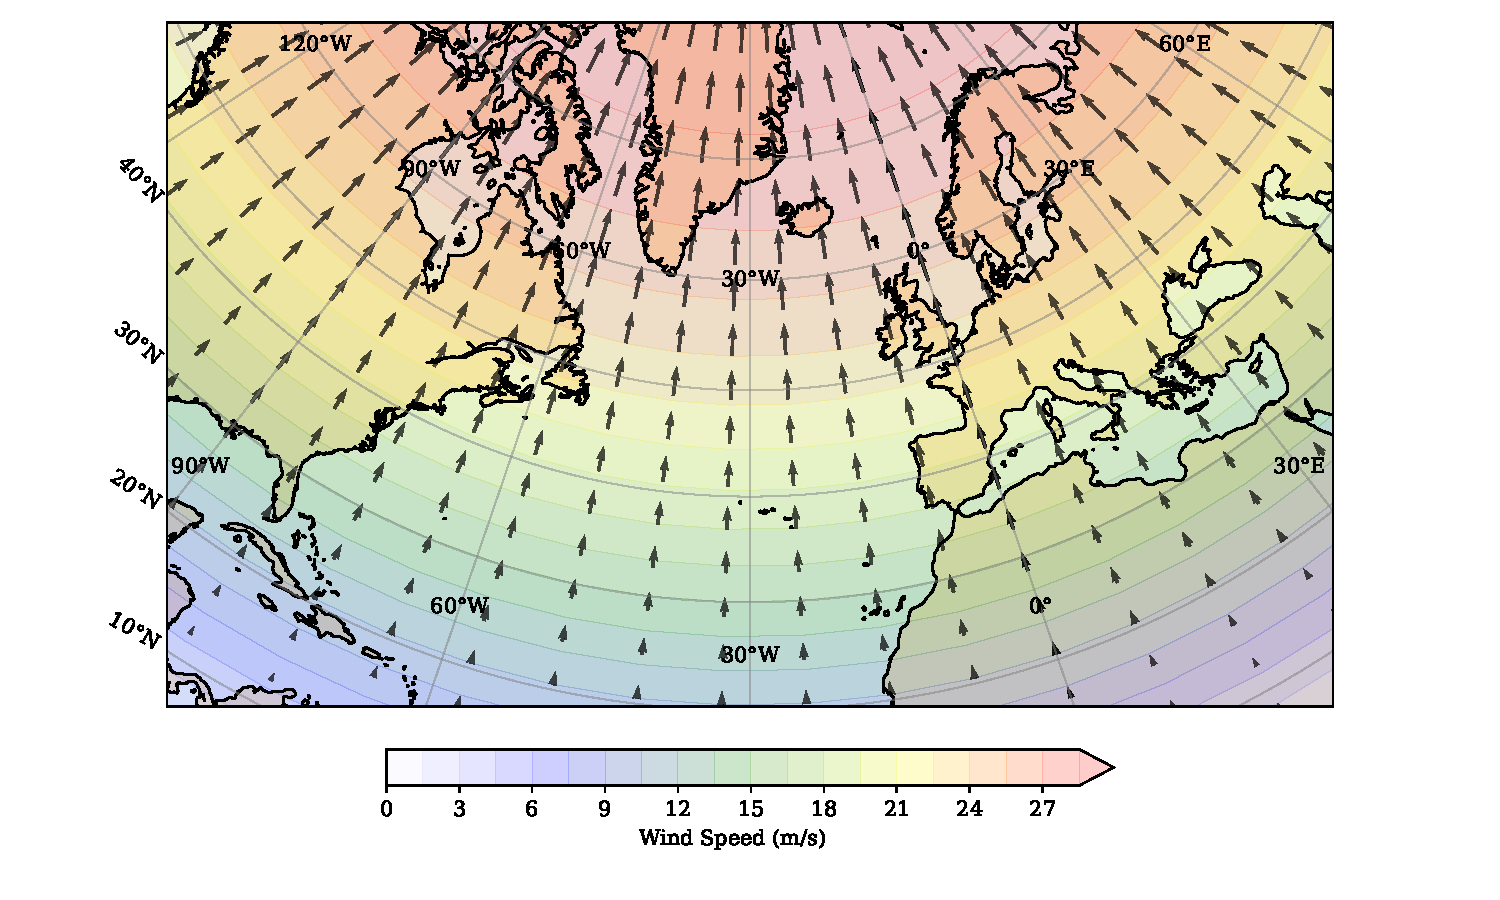
\includegraphics[width=\textwidth, trim=1cm 0cm 2cm 0cm, clip]{papers/rossby/images/meridional_wind_plot.pdf}
	\caption{Idealisiertes meridionales Windfeld (\(u=0\)), Geschwindigkeit \(v = V_0 \cdot \cos(\theta)\).}
	\label{fig:meridional_wind}
\end{figure}

\subsection{Die Drehung der Erde und die Coriolis-Kraft}

Die Erde rotiert einmal pro Tag um ihre eigene Achse. In einem rotierenden
Bezugssystem wie der Erde treten dabei Scheinkräfte auf, die in der klassischen
Mechanik berücksichtigt werden müssen. Eine davon ist die {Coriolis-Kraft},
welche bewegte Luft- und Wassermassen auf der {Nordhalbkugel} nach rechts und
auf der {Südhalbkugel} nach links ablenkt. Ihre Wirkung ist maximal an den
Polen und verschwindet am Äquator. Die Coriolis-Kraft ist keine reale Kraft,
sondern eine Folge der Drehung des Koordinatensystems.

Mathematisch wird sie beschrieben durch
\begin{equation}
	\vec{F}_C = -2m(\vec{\Omega} \times \vec{v}),
	\label{rossby:eq:coriolis_force}
\end{equation}
wobei \(m\) die Masse, \(\vec{\Omega}\) der Rotationsvektor der Erde und \(\vec{v}\) die Geschwindigkeit relativ zur Erdoberfläche ist. In atmosphärischen Anwendungen wird häufig nur die Vertikalkomponente betrachtet, was zur Definition des {Coriolis-Parameters}
\begin{equation}
	f = 2\Omega \sin(\varphi)
	\label{rossby:eq:coriolis_parameter}
\end{equation}
führt. Dessen Breitenänderung ist durch den \(\beta\)-Parameter gegeben:
\begin{equation}
	\beta = \frac{\partial f}{\partial y} = \frac{2 \Omega \cos(\varphi)}{a},
	\label{rossby:eq:beta_parameter}
\end{equation}
mit dem Erdradius \(a\) und der Nord-Süd-Koordinate \(y\).

\paragraph{Rechenbeispiel: Velofahren in Zürich}

Wir berechnen die Coriolis-Kraft auf einen Radfahrer in Zürich.

\begin{description}
	\item[Gegeben:] Geschwindigkeit \(v = 8.33\,\mathrm{m/s}\) (30\,km/h), Masse \(m =
	      80\,\mathrm{kg}\), geographische Breite \(\varphi = 47^\circ\) (Zürich),
	      Erdrotationsrate \(\Omega \approx 7.292 \times 10^{-5}\,\mathrm{rad/s}\).
	\item[Formel:]
	      \[
		      F_C = 2\,m\,v\,\Omega\,\sin(\varphi)
	      \]
	\item[Einsetzen:]
	      \[
		      F_C \approx 2 \cdot 80 \cdot 8.33 \cdot 7.292 \times 10^{-5} \cdot \sin(47^\circ)
		      \approx 0.070\,\mathrm{N}
	      \]
\end{description}

\noindent
Die resultierende Kraft von rund \(0.07\,\mathrm{N}\) ist für uns im Alltag kaum spürbar, prägt jedoch die grossräumige Atmosphärendynamik.
Sie bewirkt, dass Luftmassen nicht direkt vom Hoch- zum Tiefdruckgebiet strömen, sondern entlang der Isobaren gelenkt werden.
Dieser Effekt ist massgeblich für die Westwinddrift in den mittleren Breiten und bildet die physikalische Grundlage für Rossby-Wellen.

\subsection{Die \texorpdfstring{$\beta$}{β}-Ebene Approximation}

Die $\beta$-Ebene ist eine lokale Approximation der Erdkugel in der Umgebung
einer bestimmten geographischen Breite~$\phi_0$
(Abbildung~\ref{fig:beta_plane}). Ziel dieser Vereinfachung ist es, die
Breitenabhängigkeit der Coriolis-Kraft in mathematischen Modellen handhabbar zu
machen.
\begin{equation}
	f(y) = f_0 + \beta y,
	\label{rossby:eq:beta_plane}
\end{equation}
wobei $y$ die meridionale (Nord-Süd-)Entfernung vom Referenzbreitenkreis ist. Der Term
\begin{equation}
	f_0 = 2\Omega \sin(\phi_0)
	\label{rossby:eq:coriolis_parameter_ref}
\end{equation}
bezeichnet den Coriolisparameter an der Referenzbreite, und
\begin{equation}
	\beta = \left.\frac{\partial f}{\partial y}\right|_{\phi_0} = \frac{2\Omega \cos(\phi_0)}{a}
	\label{rossby:eq:beta_parameter_ref}
\end{equation}

beschreibt die Änderung von $f$ mit der geographischen Breite; $a$ ist der
Erdradius. Diese Darstellung erlaubt es, lokale Phänomene wie Rossby-Wellen auf
einer idealisierten Ebene zu analysieren, ohne die volle Kugelgeometrie der
Erde berücksichtigen zu müssen.

\begin{figure}
	\centering
	\begin{tikzpicture}[scale=2]
		% Tilted group (Earth and axes)
		\begin{scope}[rotate around={23.5:(0,0)}]
			% Axes
			\draw (-2,0) -- (2,0);
			\draw[->] (0,-2) -- (0,2) node[above] {Pole};

			% Earth (circle)
			\draw[thick] (1,0) arc[start angle=0, end angle=360, radius=1];

			% 3D-style spinning arrow (elliptical path)
			\draw[->, thick] ({0.3*cos(10)},{1.5 + 0.1*sin(10)})
			arc[start angle=10, end angle=320, x radius=0.3, y radius=0.1];

			% Point on the circle
			\fill[red] (30:1) circle[radius=0.05] node[right] {$P$};
			\draw[blue, thick] ($(30:1) + (120:0.5)$) -- ($(30:1) + (-60:0.5)$);
		\end{scope}
	\end{tikzpicture}
	\caption{Schematische Darstellung der $\beta$-Ebene-Approximation um einen Referenzbreitenkreis.
		Der rote Punkt \(P\) markiert die Referenzbreite, in deren Umgebung die Erdoberfläche als tangentiale Ebene angenähert wird.
		Die blaue Linie zeigt den Breitenkreis durch \(P\), der Pfeil die Rotationsrichtung der Erde.}
	\label{fig:beta_plane}
\end{figure}